\begin{figure}[htbp]
\centering
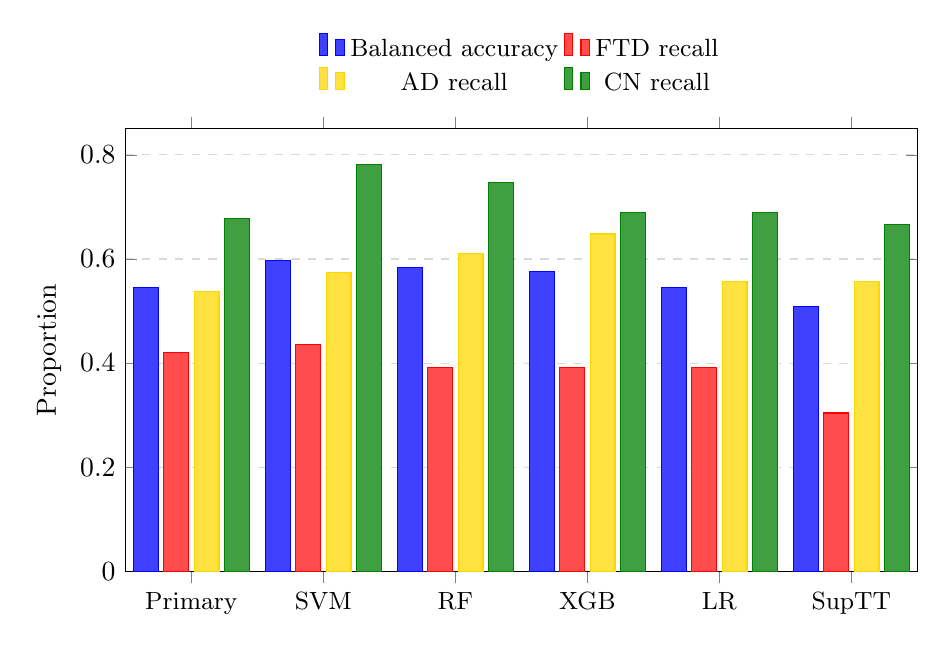
\begin{tikzpicture}
\begin{axis}[
  ybar,
  width=0.96\textwidth,
  height=72mm,
  bar width=9pt,
  ymin=0,ymax=0.85,
  ylabel={Proportion},
  symbolic x coords={Primary,SVM,RF,XGB,LR,SupTT},
  xtick=data,
  x tick label style={font=\small,rotate=0},
  ymajorgrids=true,
  grid style={dashed,gray!30},
  legend style={at={(0.5,1.23)},anchor=north,legend columns=2,draw=none,font=\small},
  enlarge x limits=0.10
]
\addplot[fill=Blue!75,draw=Blue] coordinates {(Primary,0.545) (SVM,0.597) (RF,0.583) (XGB,0.576) (LR,0.546) (SupTT,0.509)};
\addplot[fill=Red!70,draw=Red] coordinates {(Primary,0.420) (SVM,0.435) (RF,0.391) (XGB,0.391) (LR,0.391) (SupTT,0.304)};
\addplot[fill=Gold!75,draw=Gold] coordinates {(Primary,0.537) (SVM,0.574) (RF,0.611) (XGB,0.648) (LR,0.556) (SupTT,0.556)};
\addplot[fill=Green!75,draw=Green] coordinates {(Primary,0.678) (SVM,0.782) (RF,0.747) (XGB,0.690) (LR,0.690) (SupTT,0.667)};
\legend{Balanced accuracy,FTD recall,AD recall,CN recall}
\end{axis}
\end{tikzpicture}
\caption{V4 classifier-family balanced accuracy and diagnosis recall. SVM is the strongest observed family, while FTD recall remains the weakest class-specific measure.}
\label{fig:v4-classifier}
\end{figure}
